% Options for packages loaded elsewhere
\PassOptionsToPackage{unicode}{hyperref}
\PassOptionsToPackage{hyphens}{url}
\PassOptionsToPackage{dvipsnames,svgnames,x11names}{xcolor}
%
\documentclass[
  ignorenonframetext,
]{beamer}
\usepackage{pgfpages}
\setbeamertemplate{caption}[numbered]
\setbeamertemplate{caption label separator}{: }
\setbeamercolor{caption name}{fg=normal text.fg}
\beamertemplatenavigationsymbolsempty
% Prevent slide breaks in the middle of a paragraph
\widowpenalties 1 10000
\raggedbottom
\setbeamertemplate{part page}{
  \centering
  \begin{beamercolorbox}[sep=16pt,center]{part title}
    \usebeamerfont{part title}\insertpart\par
  \end{beamercolorbox}
}
\setbeamertemplate{section page}{
  \centering
  \begin{beamercolorbox}[sep=12pt,center]{part title}
    \usebeamerfont{section title}\insertsection\par
  \end{beamercolorbox}
}
\setbeamertemplate{subsection page}{
  \centering
  \begin{beamercolorbox}[sep=8pt,center]{part title}
    \usebeamerfont{subsection title}\insertsubsection\par
  \end{beamercolorbox}
}
\AtBeginPart{
  \frame{\partpage}
}
\AtBeginSection{
  \ifbibliography
  \else
    \frame{\sectionpage}
  \fi
}
\AtBeginSubsection{
  \frame{\subsectionpage}
}
\usepackage{amsmath,amssymb}
\usepackage{lmodern}
\usepackage{iftex}
\ifPDFTeX
  \usepackage[T1]{fontenc}
  \usepackage[utf8]{inputenc}
  \usepackage{textcomp} % provide euro and other symbols
\else % if luatex or xetex
  \usepackage{unicode-math}
  \defaultfontfeatures{Scale=MatchLowercase}
  \defaultfontfeatures[\rmfamily]{Ligatures=TeX,Scale=1}
\fi
% Use upquote if available, for straight quotes in verbatim environments
\IfFileExists{upquote.sty}{\usepackage{upquote}}{}
\IfFileExists{microtype.sty}{% use microtype if available
  \usepackage[]{microtype}
  \UseMicrotypeSet[protrusion]{basicmath} % disable protrusion for tt fonts
}{}
\makeatletter
\@ifundefined{KOMAClassName}{% if non-KOMA class
  \IfFileExists{parskip.sty}{%
    \usepackage{parskip}
  }{% else
    \setlength{\parindent}{0pt}
    \setlength{\parskip}{6pt plus 2pt minus 1pt}}
}{% if KOMA class
  \KOMAoptions{parskip=half}}
\makeatother
\usepackage{xcolor}
\newif\ifbibliography
\usepackage{color}
\usepackage{fancyvrb}
\newcommand{\VerbBar}{|}
\newcommand{\VERB}{\Verb[commandchars=\\\{\}]}
\DefineVerbatimEnvironment{Highlighting}{Verbatim}{commandchars=\\\{\}}
% Add ',fontsize=\small' for more characters per line
\usepackage{framed}
\definecolor{shadecolor}{RGB}{248,248,248}
\newenvironment{Shaded}{\begin{snugshade}}{\end{snugshade}}
\newcommand{\AlertTok}[1]{\textcolor[rgb]{0.94,0.16,0.16}{#1}}
\newcommand{\AnnotationTok}[1]{\textcolor[rgb]{0.56,0.35,0.01}{\textbf{\textit{#1}}}}
\newcommand{\AttributeTok}[1]{\textcolor[rgb]{0.77,0.63,0.00}{#1}}
\newcommand{\BaseNTok}[1]{\textcolor[rgb]{0.00,0.00,0.81}{#1}}
\newcommand{\BuiltInTok}[1]{#1}
\newcommand{\CharTok}[1]{\textcolor[rgb]{0.31,0.60,0.02}{#1}}
\newcommand{\CommentTok}[1]{\textcolor[rgb]{0.56,0.35,0.01}{\textit{#1}}}
\newcommand{\CommentVarTok}[1]{\textcolor[rgb]{0.56,0.35,0.01}{\textbf{\textit{#1}}}}
\newcommand{\ConstantTok}[1]{\textcolor[rgb]{0.00,0.00,0.00}{#1}}
\newcommand{\ControlFlowTok}[1]{\textcolor[rgb]{0.13,0.29,0.53}{\textbf{#1}}}
\newcommand{\DataTypeTok}[1]{\textcolor[rgb]{0.13,0.29,0.53}{#1}}
\newcommand{\DecValTok}[1]{\textcolor[rgb]{0.00,0.00,0.81}{#1}}
\newcommand{\DocumentationTok}[1]{\textcolor[rgb]{0.56,0.35,0.01}{\textbf{\textit{#1}}}}
\newcommand{\ErrorTok}[1]{\textcolor[rgb]{0.64,0.00,0.00}{\textbf{#1}}}
\newcommand{\ExtensionTok}[1]{#1}
\newcommand{\FloatTok}[1]{\textcolor[rgb]{0.00,0.00,0.81}{#1}}
\newcommand{\FunctionTok}[1]{\textcolor[rgb]{0.00,0.00,0.00}{#1}}
\newcommand{\ImportTok}[1]{#1}
\newcommand{\InformationTok}[1]{\textcolor[rgb]{0.56,0.35,0.01}{\textbf{\textit{#1}}}}
\newcommand{\KeywordTok}[1]{\textcolor[rgb]{0.13,0.29,0.53}{\textbf{#1}}}
\newcommand{\NormalTok}[1]{#1}
\newcommand{\OperatorTok}[1]{\textcolor[rgb]{0.81,0.36,0.00}{\textbf{#1}}}
\newcommand{\OtherTok}[1]{\textcolor[rgb]{0.56,0.35,0.01}{#1}}
\newcommand{\PreprocessorTok}[1]{\textcolor[rgb]{0.56,0.35,0.01}{\textit{#1}}}
\newcommand{\RegionMarkerTok}[1]{#1}
\newcommand{\SpecialCharTok}[1]{\textcolor[rgb]{0.00,0.00,0.00}{#1}}
\newcommand{\SpecialStringTok}[1]{\textcolor[rgb]{0.31,0.60,0.02}{#1}}
\newcommand{\StringTok}[1]{\textcolor[rgb]{0.31,0.60,0.02}{#1}}
\newcommand{\VariableTok}[1]{\textcolor[rgb]{0.00,0.00,0.00}{#1}}
\newcommand{\VerbatimStringTok}[1]{\textcolor[rgb]{0.31,0.60,0.02}{#1}}
\newcommand{\WarningTok}[1]{\textcolor[rgb]{0.56,0.35,0.01}{\textbf{\textit{#1}}}}
\usepackage{graphicx}
\makeatletter
\def\maxwidth{\ifdim\Gin@nat@width>\linewidth\linewidth\else\Gin@nat@width\fi}
\def\maxheight{\ifdim\Gin@nat@height>\textheight\textheight\else\Gin@nat@height\fi}
\makeatother
% Scale images if necessary, so that they will not overflow the page
% margins by default, and it is still possible to overwrite the defaults
% using explicit options in \includegraphics[width, height, ...]{}
\setkeys{Gin}{width=\maxwidth,height=\maxheight,keepaspectratio}
% Set default figure placement to htbp
\makeatletter
\def\fps@figure{htbp}
\makeatother
\setlength{\emergencystretch}{3em} % prevent overfull lines
\providecommand{\tightlist}{%
  \setlength{\itemsep}{0pt}\setlength{\parskip}{0pt}}
\setcounter{secnumdepth}{-\maxdimen} % remove section numbering
\usepackage{graphicx}
\usepackage{bm}
\usepackage{array}
\usepackage{amsmath}
\usepackage{amsthm}
\usepackage{amsfonts}
\usepackage{amssymb}
\usepackage{tikz-cd}
\usepackage{url}
\definecolor{foreground}{RGB}{255,255,255}
\definecolor{background}{RGB}{34,28,54}
\definecolor{title}{RGB}{105,165,255}
\definecolor{gray}{RGB}{175,175,175}
\definecolor{lightgray}{RGB}{225,225,225}
\definecolor{subtitle}{RGB}{232,234,255}
\definecolor{hilight}{RGB}{112,224,255}
\definecolor{vhilight}{RGB}{255,111,207}
\setbeamertemplate{footline}[page number]
\ifLuaTeX
  \usepackage{selnolig}  % disable illegal ligatures
\fi
\IfFileExists{bookmark.sty}{\usepackage{bookmark}}{\usepackage{hyperref}}
\IfFileExists{xurl.sty}{\usepackage{xurl}}{} % add URL line breaks if available
\urlstyle{same} % disable monospaced font for URLs
\hypersetup{
  pdftitle={STAT 528 - Advanced Regression Analysis II},
  pdfauthor={Count response regression (part I)},
  colorlinks=true,
  linkcolor={Maroon},
  filecolor={Maroon},
  citecolor={Blue},
  urlcolor={blue},
  pdfcreator={LaTeX via pandoc}}

\title{STAT 528 - Advanced Regression Analysis II}
\author{Count response regression (part I)}
\date{}
\institute{Daniel J. Eck\\
Department of Statistics\\
University of Illinois}

\begin{document}
\frame{\titlepage}

\begin{frame}
\newcommand{\R}{\mathbb{R}}
\newcommand{\Prob}{\mathbb{P}}
\newcommand{\Proj}{\textbf{P}}
\newcommand{\Hcal}{\mathcal{H}}
\newcommand{\rootn}{\sqrt{n}}
\newcommand{\p}{\mathbf{p}}
\newcommand{\E}{\text{E}}
\newcommand{\Var}{\text{Var}}
\newcommand{\Cov}{\text{Cov}}
\newcommand{\mubf}{\bm{\mu}}
\newcommand{\logit}{\text{logit}}

\newtheorem{cor}{Corollary}
\newtheorem{lem}{Lemma}
\newtheorem{thm}{Theorem}
\newtheorem{defn}{Definition}
\newtheorem{prop}{Proposition}
\end{frame}

\begin{frame}{Last time}
\protect\hypertarget{last-time}{}
\begin{itemize}
\tightlist
\item
  basic diagnostics for binary response models
\item
  probit regression and threshold modeling
\item
  basic causal inference
\end{itemize}
\end{frame}

\begin{frame}{Learning Objectives Today}
\protect\hypertarget{learning-objectives-today}{}
\begin{itemize}
\tightlist
\item
  Poisson regression
\item
  Residual diagnostics
\item
  Data analysis
\end{itemize}
\end{frame}

\begin{frame}{Background (again)}
\protect\hypertarget{background-again}{}
We suppose that we have a sample of data \((y_i,x_i)\),
\(i = 1,\ldots, n\) where

\begin{itemize}
\tightlist
\item
  \(y_i\) is a scalar response variable
\item
  \(x_i\) is a vector of predictors.
\end{itemize}

Recall from the exponential family notes that the log likelihood of the
exponential family is of the form \begin{equation} \label{expolog}
    l(\theta) = \langle y, \theta \rangle - c(\theta),
\end{equation} where

\begin{itemize}
\tightlist
\item
  \(y \in \mathbb{R}^n\) is a vector statistic having components
\item
  \(\theta \in \mathbb{R}^n\) is the canonical parameter vector.
\end{itemize}

In those notes \(\theta\) is unconstrained and the likelihood
\eqref{expolog} corresponds to a saturated regression model, one
parameter for every observation.
\end{frame}

\begin{frame}{}
\protect\hypertarget{section}{}
A canonical linear submodel of an exponential family is a submodel
having parameterization \[
  \theta = M\beta,
\] and log likelihood \begin{equation} \label{subloglike}
  l(\beta) = \langle M'y, \beta \rangle - c(M\beta).
\end{equation}

In an exponential family GLM, the saturated model canonical parameter
vector \(\theta\) is ``linked'\,' to the saturated model mean value
parameter vector through the change-of-parameter mappings \(g(\theta)\).

\vspace{12pt}

We can write \[
 \mu = \text{E}_\theta(Y) = g(M\beta) 
\] which implies that we can write \[
  g^{-1}\left(\text{E}_\theta(Y)\right) = M\beta.
\]
\end{frame}

\begin{frame}{Poisson regression model}
\protect\hypertarget{poisson-regression-model}{}
The Poisson regression model {[}and its variants{]} is one of the more
widely used and studied exponential family GLMs in practice.

\vspace{12pt}

The Poisson regression model is used for analyzing a count response
variable, \(y_i \in \{0,1,2,\ldots\}\).

\vspace{12pt}

The Poisson regression model allows for users to model expected counts
as a function of covariates.
\end{frame}

\begin{frame}{preliminaries}
\protect\hypertarget{preliminaries}{}
Recall the Poisson distributions with mass function \[
  P(Y = y) = \frac{\mu^ye^{-\mu}}{y!}, \qquad (y = 0,1,2,\ldots),
\] where \(E(Y) = \mu\) and Var\((Y) = \mu\).
\end{frame}

\begin{frame}{}
\protect\hypertarget{section-1}{}
For a count response variable \(Y\) and a vector of predictors \(X\),
let \(\mu(x) = \text{E}(Y|X = x)\). The Poisson regression model is then
\begin{equation} \label{loglink}
  \mu(x) = \text{E}(Y|X = x) = \exp\left(x'\beta\right).
\end{equation} Equivalently, \[
  \log\left(\mu(x)\right) = x'\beta.
\] In vector notation, we can express the above as \[
  \bm{\mu}= \exp(M\beta) \quad \text{and} \quad \text{log}(\bm{\mu}) = M\beta
\] where the above \(\exp(\cdot)\) and log\((\cdot)\) operations are
understood as componentwise operations.
\end{frame}

\begin{frame}{}
\protect\hypertarget{section-2}{}
Let's consider the log likelihood of a sample of independent Poisson
random variables \begin{align*}
  \sum_{i=1}^n y_i\log(\mu_i) - \mu_i 
    &=  \sum_{i=1}^n y_i\theta_i - \exp(\theta_i)
\end{align*} where \[
  \theta_i = \log\left(\mu_i\right) = g^{-1}(\mu_i) \qquad \text{and} \qquad \mu_i = \exp(\theta_i) = g(\theta_i).
\]

We see that the Poisson regression model with log link is a canonical
linear submodel of an exponential family when we write \[
  \theta_i = x_i'\beta.
\]
\end{frame}

\begin{frame}{Example: Gala data}
\protect\hypertarget{example-gala-data}{}
We will demonstrate Poisson regression modeling on the Galapagos data
frame in the \texttt{faraway} package. This data frame consists of
\(n = 30\) observations and \(7\) variables in total.

\vspace{12pt}

For 30 Galapagos Islands, we have:

\begin{itemize}
\tightlist
\item
  a count of the number of plant species found on each island
\item
  five geographic variables for each island
\end{itemize}

\vspace{12pt}

A few missing values have been filled in for simplicity. We will model
the number of species using Poisson regression using the glm function in
R.
\end{frame}

\begin{frame}{Galapagos variables}
\protect\hypertarget{galapagos-variables}{}
\begin{itemize}
\tightlist
\item
  \textbf{Species}: the number of plant species found on the island
\item
  \textbf{Area}: the area of the island (km\(^2\))
\item
  \textbf{Elevation}: the highest elevation of the island (m)
\item
  \textbf{Nearest}: the distance from the nearest island (km)
\item
  \textbf{Scruz}: the distance from Santa Cruz island (km)
\item
  \textbf{Adjacent}: the area of the adjacent island (square km)
\end{itemize}

\vspace{12pt}

M. P. Johnson and P. H. Raven (1973)
``\href{https://pubmed.ncbi.nlm.nih.gov/17832770/}{Species number and
endemism: The Galapagos Archipelago revisited}'' Science, 179, 893-895
\end{frame}

\begin{frame}[fragile]{}
\protect\hypertarget{section-3}{}
We first load in necessary software.

\vspace{12pt}
\small

\begin{Shaded}
\begin{Highlighting}[]
\FunctionTok{rm}\NormalTok{(}\AttributeTok{list =} \FunctionTok{ls}\NormalTok{())}
\FunctionTok{library}\NormalTok{(tidyverse)}
\FunctionTok{library}\NormalTok{(faraway)}
\end{Highlighting}
\end{Shaded}

\vspace{12pt}

We create a discrete size variable based on the Area variable for
demonstration purposes, and then fit the Poisson regression model

\vspace{12pt}
\footnotesize

\begin{Shaded}
\begin{Highlighting}[]
\NormalTok{gala }\OtherTok{\textless{}{-}}\NormalTok{ gala }\SpecialCharTok{\%\textgreater{}\%} 
  \FunctionTok{mutate}\NormalTok{(}\AttributeTok{Size =} \FunctionTok{as.factor}\NormalTok{(}\DecValTok{1} \SpecialCharTok{+} \FunctionTok{ifelse}\NormalTok{(Area }\SpecialCharTok{\textgreater{}} \DecValTok{1}\NormalTok{,}\DecValTok{1}\NormalTok{,}\DecValTok{0}\NormalTok{) }\SpecialCharTok{+} 
                            \FunctionTok{ifelse}\NormalTok{(Area }\SpecialCharTok{\textgreater{}} \DecValTok{25}\NormalTok{,}\DecValTok{1}\NormalTok{,}\DecValTok{0}\NormalTok{)))}
\NormalTok{m1 }\OtherTok{\textless{}{-}} \FunctionTok{glm}\NormalTok{(Species }\SpecialCharTok{\textasciitilde{}}\NormalTok{ Elevation }\SpecialCharTok{+}\NormalTok{ Nearest }\SpecialCharTok{+}\NormalTok{ Scruz }\SpecialCharTok{+}\NormalTok{ Adjacent }\SpecialCharTok{+}\NormalTok{ Size, }
          \AttributeTok{family =} \StringTok{"poisson"}\NormalTok{, }\AttributeTok{data =}\NormalTok{ gala, }\AttributeTok{x =} \ConstantTok{TRUE}\NormalTok{)}
\end{Highlighting}
\end{Shaded}
\end{frame}

\begin{frame}{}
\protect\hypertarget{section-4}{}
As in logistic regression, we are going to unpack the glm call.

\vspace{12pt}

The specific log likelihood for the Poisson regression model is \[
  l(\beta) \propto \sum_{i=1}^n y_ix_i'\beta - \exp\left(x_i'\beta\right)
\] where

\begin{itemize}
\tightlist
\item
  \(x_i'\)s are the rows of the design matrix \(M\)
\item
  \(y_i\)s are the components of the response vector \(y\) (the Species
  variable corresponding to the number of species on each of the
  islands)
\item
  \(\beta\) is the submodel canonical parameter vector
\end{itemize}

\vspace{12pt}

The glm function then performs a Fisher scoring based optimization
routine to maximize the above likelihood.
\end{frame}

\begin{frame}[fragile]{}
\protect\hypertarget{section-5}{}
We can view summary information for \(\hat\beta\) and the fitting
process using the summary function

\tiny

\begin{Shaded}
\begin{Highlighting}[]
\FunctionTok{summary}\NormalTok{(m1)}
\end{Highlighting}
\end{Shaded}

\begin{verbatim}
## 
## Call:
## glm(formula = Species ~ Elevation + Nearest + Scruz + Adjacent + 
##     Size, family = "poisson", data = gala, x = TRUE)
## 
## Deviance Residuals: 
##      Min        1Q    Median        3Q       Max  
## -10.3723   -3.5214   -0.9947    1.7193   10.6627  
## 
## Coefficients:
##               Estimate Std. Error z value Pr(>|z|)    
## (Intercept)  2.790e+00  8.108e-02  34.410  < 2e-16 ***
## Elevation    9.361e-04  5.402e-05  17.329  < 2e-16 ***
## Nearest      6.469e-03  1.748e-03   3.702 0.000214 ***
## Scruz       -6.266e-03  6.268e-04  -9.997  < 2e-16 ***
## Adjacent    -2.858e-04  2.961e-05  -9.652  < 2e-16 ***
## Size2        1.128e+00  9.535e-02  11.826  < 2e-16 ***
## Size3        2.059e+00  9.419e-02  21.856  < 2e-16 ***
## ---
## Signif. codes:  0 '***' 0.001 '**' 0.01 '*' 0.05 '.' 0.1 ' ' 1
## 
## (Dispersion parameter for poisson family taken to be 1)
## 
##     Null deviance: 3510.73  on 29  degrees of freedom
## Residual deviance:  594.18  on 23  degrees of freedom
## AIC: 769.01
## 
## Number of Fisher Scoring iterations: 5
\end{verbatim}
\end{frame}

\begin{frame}{}
\protect\hypertarget{section-6}{}
Keep in mind that interpretations of \(\beta\) are on the log scale.

\vspace{12pt}

A particular component of \(\hat{\beta}\) gives the estimated change in
logs of expected counts when one makes a unit change to a particular
component of the covariate vector with all other components held fixed.

\vspace{12pt}

Similar story for logistic regression. A particular component of
\(\hat{\beta}\) gives the estimated change in log odds when one makes a
unit change to a particular component of the covariate vector with all
other components held fixed.

\vspace{12pt}

This is good to keep in mind and it \emph{may} be instructive for how
you answer homework questions. But keep in mind that:

\begin{itemize}
\tightlist
\item
  \(\beta\) is given by \(M\) and not span\((M)\)
\item
  modeling of expectations is the motivation for these models
\end{itemize}
\end{frame}

\begin{frame}[fragile]{Demonstration of this point}
\protect\hypertarget{demonstration-of-this-point}{}
\tiny

\begin{Shaded}
\begin{Highlighting}[]
\NormalTok{m2 }\OtherTok{\textless{}{-}}  \FunctionTok{glm}\NormalTok{(Species }\SpecialCharTok{\textasciitilde{}} \SpecialCharTok{{-}}\DecValTok{1} \SpecialCharTok{+}\NormalTok{ Elevation }\SpecialCharTok{+}\NormalTok{ Nearest }\SpecialCharTok{+}\NormalTok{ Scruz }\SpecialCharTok{+}\NormalTok{ Adjacent }\SpecialCharTok{+}\NormalTok{ Size, }
          \AttributeTok{family =} \StringTok{"poisson"}\NormalTok{, }\AttributeTok{data =}\NormalTok{ gala, }\AttributeTok{x =} \ConstantTok{TRUE}\NormalTok{)}
\FunctionTok{summary}\NormalTok{(m2)}
\end{Highlighting}
\end{Shaded}

\begin{verbatim}
## 
## Call:
## glm(formula = Species ~ -1 + Elevation + Nearest + Scruz + Adjacent + 
##     Size, family = "poisson", data = gala, x = TRUE)
## 
## Deviance Residuals: 
##      Min        1Q    Median        3Q       Max  
## -10.3723   -3.5214   -0.9947    1.7193   10.6627  
## 
## Coefficients:
##             Estimate Std. Error z value Pr(>|z|)    
## Elevation  9.361e-04  5.402e-05  17.329  < 2e-16 ***
## Nearest    6.469e-03  1.748e-03   3.702 0.000214 ***
## Scruz     -6.266e-03  6.268e-04  -9.997  < 2e-16 ***
## Adjacent  -2.858e-04  2.961e-05  -9.652  < 2e-16 ***
## Size1      2.790e+00  8.108e-02  34.410  < 2e-16 ***
## Size2      3.917e+00  5.761e-02  68.001  < 2e-16 ***
## Size3      4.848e+00  5.987e-02  80.990  < 2e-16 ***
## ---
## Signif. codes:  0 '***' 0.001 '**' 0.01 '*' 0.05 '.' 0.1 ' ' 1
## 
## (Dispersion parameter for poisson family taken to be 1)
## 
##     Null deviance: 21190.47  on 30  degrees of freedom
## Residual deviance:   594.18  on 23  degrees of freedom
## AIC: 769.01
## 
## Number of Fisher Scoring iterations: 5
\end{verbatim}
\end{frame}

\begin{frame}[fragile]{}
\protect\hypertarget{section-7}{}
We see that

\vspace{12pt}

\begin{Shaded}
\begin{Highlighting}[]
\FunctionTok{logLik}\NormalTok{(m1) }\SpecialCharTok{{-}} \FunctionTok{logLik}\NormalTok{(m2)}
\end{Highlighting}
\end{Shaded}

\begin{verbatim}
## 'log Lik.' 5.684342e-14 (df=7)
\end{verbatim}

\vspace{12pt}
\normalsize

and

\vspace{12pt}
\footnotesize

\begin{Shaded}
\begin{Highlighting}[]
\NormalTok{theta1 }\OtherTok{\textless{}{-}}\NormalTok{ m1}\SpecialCharTok{$}\NormalTok{x }\SpecialCharTok{\%*\%} \FunctionTok{coef}\NormalTok{(m1)}
\NormalTok{theta2 }\OtherTok{\textless{}{-}}\NormalTok{ m2}\SpecialCharTok{$}\NormalTok{x }\SpecialCharTok{\%*\%} \FunctionTok{coef}\NormalTok{(m2)}
\FunctionTok{all.equal}\NormalTok{(theta1, theta2)}
\end{Highlighting}
\end{Shaded}

\begin{verbatim}
## [1] TRUE
\end{verbatim}
\end{frame}

\begin{frame}[fragile]{}
\protect\hypertarget{section-8}{}
However, \(\hat{\beta}_1 \neq \hat{\beta}_2\)

\vspace{12pt}
\tiny

\begin{Shaded}
\begin{Highlighting}[]
\FunctionTok{coef}\NormalTok{(m1)}
\end{Highlighting}
\end{Shaded}

\begin{verbatim}
##   (Intercept)     Elevation       Nearest         Scruz      Adjacent 
##  2.7897964708  0.0009360990  0.0064693041 -0.0062664946 -0.0002857805 
##         Size2         Size3 
##  1.1276155398  2.0586771298
\end{verbatim}

\begin{Shaded}
\begin{Highlighting}[]
\FunctionTok{coef}\NormalTok{(m2)}
\end{Highlighting}
\end{Shaded}

\begin{verbatim}
##     Elevation       Nearest         Scruz      Adjacent         Size1 
##  0.0009360990  0.0064693041 -0.0062664946 -0.0002857805  2.7897964708 
##         Size2         Size3 
##  3.9174120106  4.8484736007
\end{verbatim}
\end{frame}

\begin{frame}{Other parameterizations}
\protect\hypertarget{other-parameterizations}{}
Recall:

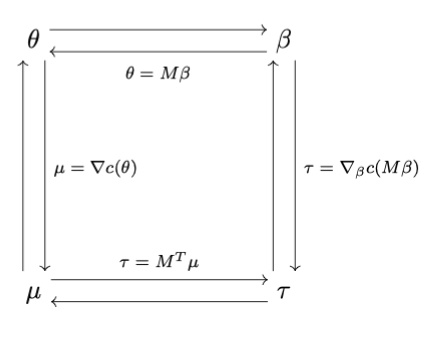
\includegraphics{transformations.png}
\end{frame}

\begin{frame}[fragile]{}
\protect\hypertarget{section-9}{}
We start with \[
  \langle M'y, \beta \rangle - c_\beta(\beta),
\] and then obtain \(\hat{\beta}\) by maximizing the above. From here:

\begin{itemize}
\tightlist
\item
  \(\hat{\theta} = M\hat{\beta}\)
\item
  \(\hat\mu = \nabla_\theta c(\theta^*)|_{\theta* = \hat{\theta}}\)
\item
  \(\hat\tau = M'\hat{u}\)
\end{itemize}

\vspace{12pt}

For example we can compute \(\hat\theta\) using the predict function or
by hand. \vspace{12pt} \tiny

\begin{Shaded}
\begin{Highlighting}[]
\NormalTok{theta }\OtherTok{\textless{}{-}}\NormalTok{ m1}\SpecialCharTok{$}\NormalTok{x }\SpecialCharTok{\%*\%} \FunctionTok{coef}\NormalTok{(m1)}
\FunctionTok{head}\NormalTok{(}\FunctionTok{cbind}\NormalTok{(}\FunctionTok{predict}\NormalTok{(m1, }\AttributeTok{type =} \StringTok{"link"}\NormalTok{), theta), }\DecValTok{3}\NormalTok{)}
\end{Highlighting}
\end{Shaded}

\begin{verbatim}
##               [,1]     [,2]
## Baltra    5.171960 5.171960
## Bartolome 3.694959 3.694959
## Caldwell  2.546560 2.546560
\end{verbatim}
\end{frame}

\begin{frame}{Inference}
\protect\hypertarget{inference}{}
The standard error column of the summary table are estimates of the
square root of the variances of the estimated submodel canonical
statistic vector \(\hat\beta\).

\vspace{12pt}

Recall from the asymptotic theory of MLE that \[
  \sqrt{n}(\hat\beta - \beta) \overset{d}{\to} N(0, \Sigma^{-1}),
\] where \(\Sigma^{-1}\) is the inverse of the Fisher information
matrix.
\end{frame}

\begin{frame}[fragile]{}
\protect\hypertarget{section-10}{}
We can extract these same standard errors using the vcov function

\vspace{12pt}
\tiny

\begin{Shaded}
\begin{Highlighting}[]
\FunctionTok{sqrt}\NormalTok{(}\FunctionTok{diag}\NormalTok{(}\FunctionTok{vcov}\NormalTok{(m1)))}
\end{Highlighting}
\end{Shaded}

\begin{verbatim}
##  (Intercept)    Elevation      Nearest        Scruz     Adjacent        Size2 
## 8.107577e-02 5.402068e-05 1.747556e-03 6.268325e-04 2.960794e-05 9.535081e-02 
##        Size3 
## 9.419199e-02
\end{verbatim}

\vspace{12pt}
\normalsize

These values are the same as those in the Std. Error column in the above
summary table

\vspace{12pt}
\tiny

\begin{Shaded}
\begin{Highlighting}[]
\FunctionTok{all.equal}\NormalTok{(}\FunctionTok{summary}\NormalTok{(m1)}\SpecialCharTok{$}\NormalTok{coef[, }\DecValTok{2}\NormalTok{], }\FunctionTok{sqrt}\NormalTok{(}\FunctionTok{diag}\NormalTok{(}\FunctionTok{vcov}\NormalTok{(m1))))}
\end{Highlighting}
\end{Shaded}

\begin{verbatim}
## [1] TRUE
\end{verbatim}
\end{frame}

\begin{frame}{}
\protect\hypertarget{section-11}{}
We can make inferences about \(\beta_j\) using the Wald statistic
corresponding to the hypothesis test \[
  H_o: \beta_j = 0, \qquad H_a:\beta_j \neq 0,
\] which is given by \[
  \frac{\hat{\beta_j}}{\text{se}(\hat\beta_j)} \sim N(0,1),
\] where this distributional relationship holds under the null
hypothesis \(\beta_j = 0\). Similarly, we can form a confidence interval
\[
  \hat\beta_j \pm z_{\alpha/2}\text{se}(\hat\beta_j)
\] where \(0 < \alpha < 1\) is some error threshold.
\end{frame}

\begin{frame}{Deviance and likelihood ratio testing}
\protect\hypertarget{deviance-and-likelihood-ratio-testing}{}
Recall our \(l(\mu;y)\) notation.

\vspace{12pt}

The deviance is defined by \[
 -2\left[l(\hat\mu;y) - l(y;y)\right].
\] This is the likelihood-ratio for testing the null hypothesis that the
model against the general alternative (ie, the saturated model). The
deviance has reference distribution \[
  -2\left[l(\hat\mu;y) - l(y;y)\right] \approx \chi^2_{\text{df}}
\] where df = \(n - p\), \(n\) is the sample size, and \(p\) is the
number of model parameters.
\end{frame}

\begin{frame}{}
\protect\hypertarget{section-12}{}
We can also test nested models using deviance based testing \[
  -2\left[l(\hat\mu_1;y) - l(\hat\mu_2;y)\right] \approx \chi^2_{\text{df}}
\] where

\begin{itemize}
\tightlist
\item
  \(\hat{\mu_1}\) corresponds to a smaller model than that which led to
  estimation of \(\hat{\mu}_2\)
\item
  df = \(p_1 - p_2\)
\end{itemize}
\end{frame}

\begin{frame}[fragile]{}
\protect\hypertarget{section-13}{}
Let's consider the smaller model that ignores the Elevation variable. A
likelihood ratio test shows that the larger model is preferable at any
reasonably chosen significance level \(\alpha\).

\vspace{12pt}
\tiny

\begin{Shaded}
\begin{Highlighting}[]
\NormalTok{m\_small }\OtherTok{\textless{}{-}} \FunctionTok{glm}\NormalTok{(Species }\SpecialCharTok{\textasciitilde{}}\NormalTok{ Nearest }\SpecialCharTok{+}\NormalTok{ Scruz }\SpecialCharTok{+}\NormalTok{ Adjacent }\SpecialCharTok{+}\NormalTok{ Size, }
          \AttributeTok{family =} \StringTok{"poisson"}\NormalTok{, }\AttributeTok{data =}\NormalTok{ gala, }\AttributeTok{x =} \ConstantTok{TRUE}\NormalTok{)}

\DocumentationTok{\#\# built in likelihood ratio test using anova.glm}
\FunctionTok{anova}\NormalTok{(m\_small, m1, }\AttributeTok{test =} \StringTok{"LRT"}\NormalTok{)}
\end{Highlighting}
\end{Shaded}

\begin{verbatim}
## Analysis of Deviance Table
## 
## Model 1: Species ~ Nearest + Scruz + Adjacent + Size
## Model 2: Species ~ Elevation + Nearest + Scruz + Adjacent + Size
##   Resid. Df Resid. Dev Df Deviance  Pr(>Chi)    
## 1        24     878.14                          
## 2        23     594.18  1   283.96 < 2.2e-16 ***
## ---
## Signif. codes:  0 '***' 0.001 '**' 0.01 '*' 0.05 '.' 0.1 ' ' 1
\end{verbatim}

\begin{Shaded}
\begin{Highlighting}[]
\DocumentationTok{\#\# perform the above directly (different machine tolerances)}
\FunctionTok{pchisq}\NormalTok{(m\_small}\SpecialCharTok{$}\NormalTok{deviance }\SpecialCharTok{{-}}\NormalTok{ m1}\SpecialCharTok{$}\NormalTok{deviance, }\AttributeTok{df =} \DecValTok{1}\NormalTok{, }\AttributeTok{lower =} \ConstantTok{FALSE}\NormalTok{)}
\end{Highlighting}
\end{Shaded}

\begin{verbatim}
## [1] 1.029422e-63
\end{verbatim}
\end{frame}

\begin{frame}{}
\protect\hypertarget{section-14}{}
In this example we see that the levels of the Size variable are
statistically significant at any reasonable error threshold \(\alpha\).

\vspace{12pt}

Suppose instead that we wanted to test if large islands are expected to
have a different number of species than medium sized islands.

\vspace{12pt}

Informally, the summary table above suggests that large islands have
mores species than medium sized islands, but this is not a formal
comparison.

\vspace{12pt}

Formally, we want to test \[
  H_o: \mu_l - \mu_m = 0, \qquad H_a: \mu_l - \mu_m \neq 0,
\] where \(\mu_l\) and \(\mu_m\), respectively, correspond to the
mean-value parameters for large and medium-sized islands.
\end{frame}

\begin{frame}{}
\protect\hypertarget{section-15}{}
We know that \(\mu_l = \exp(\beta_l)\) and \(\mu_m = \exp(\beta_m)\)
where \(\beta_l\) and \(\beta_m\), respectively, correspond to the
canonical parameters for large and medium-sized islands.

\vspace{12pt}

We can test the hypothesis on the previous slide using the Delta method
\[
  \sqrt{n}\left[ (\hat\mu_l - \hat\mu_m) - (\mu_l - \mu_m)  \right] 
    \overset{d}{\to} N\left(0, \nabla h(\beta)'\Sigma^{-1}\nabla h(\beta)\right)
\] where \[
  h(\beta) = \exp(\beta_l) - \exp(\beta_m) = \mu_l - \mu_m.
\]
\end{frame}

\begin{frame}[fragile]{}
\protect\hypertarget{section-16}{}
We obtain the estimate \(\hat\mu_l - \hat\mu_m\) below

\vspace{12pt}
\tiny

\begin{Shaded}
\begin{Highlighting}[]
\NormalTok{comp }\OtherTok{\textless{}{-}} \FunctionTok{c}\NormalTok{(}\DecValTok{0}\NormalTok{,}\DecValTok{0}\NormalTok{,}\DecValTok{0}\NormalTok{,}\DecValTok{0}\NormalTok{,}\DecValTok{0}\NormalTok{,}\SpecialCharTok{{-}}\DecValTok{1}\NormalTok{,}\DecValTok{1}\NormalTok{)}
\NormalTok{betahat }\OtherTok{\textless{}{-}}\NormalTok{ m1}\SpecialCharTok{$}\NormalTok{coefficients}
\NormalTok{grad }\OtherTok{\textless{}{-}} \FunctionTok{exp}\NormalTok{(betahat) }\SpecialCharTok{*}\NormalTok{ comp}
\NormalTok{est }\OtherTok{\textless{}{-}} \FunctionTok{sum}\NormalTok{(grad)}
\NormalTok{est}
\end{Highlighting}
\end{Shaded}

\begin{verbatim}
## [1] 4.747314
\end{verbatim}

\vspace{12pt}
\normalsize

and the estimate of \(\nabla h(\beta)\) is the column vector below

\vspace{12pt}
\tiny

\begin{Shaded}
\begin{Highlighting}[]
\NormalTok{grad}
\end{Highlighting}
\end{Shaded}

\begin{verbatim}
## (Intercept)   Elevation     Nearest       Scruz    Adjacent       Size2 
##    0.000000    0.000000    0.000000    0.000000    0.000000   -3.088284 
##       Size3 
##    7.835597
\end{verbatim}
\end{frame}

\begin{frame}[fragile]{}
\protect\hypertarget{section-17}{}
The asymptotic variance \(\nabla h(\beta)^T\Sigma^{-1}\nabla h(\beta)\)
and corresponding standard error are estimated below

\vspace{12pt}
\tiny

\begin{Shaded}
\begin{Highlighting}[]
\NormalTok{InvFish }\OtherTok{\textless{}{-}} \FunctionTok{vcov}\NormalTok{(m1)}
\NormalTok{asympVar }\OtherTok{\textless{}{-}} \FunctionTok{as.numeric}\NormalTok{(}\FunctionTok{t}\NormalTok{(grad) }\SpecialCharTok{\%*\%}\NormalTok{ InvFish }\SpecialCharTok{\%*\%}\NormalTok{ grad)}
\NormalTok{asympVar}
\end{Highlighting}
\end{Shaded}

\begin{verbatim}
## [1] 0.2965522
\end{verbatim}

\begin{Shaded}
\begin{Highlighting}[]
\NormalTok{SE }\OtherTok{\textless{}{-}} \FunctionTok{sqrt}\NormalTok{(asympVar)}
\NormalTok{SE}
\end{Highlighting}
\end{Shaded}

\begin{verbatim}
## [1] 0.5445661
\end{verbatim}

\vspace{12pt}
\normalsize

The ratio \((\hat\mu_l - \hat\mu_m)/\text{se}(\hat\mu_l - \hat\mu_m)\)
is given by

\vspace{12pt}
\tiny

\begin{Shaded}
\begin{Highlighting}[]
\NormalTok{est}\SpecialCharTok{/}\NormalTok{SE}
\end{Highlighting}
\end{Shaded}

\begin{verbatim}
## [1] 8.717608
\end{verbatim}

\vspace{12pt}
\normalsize

and a corresponding 95\% confidence interval is

\vspace{12pt}
\tiny

\begin{Shaded}
\begin{Highlighting}[]
\NormalTok{est }\SpecialCharTok{+} \FunctionTok{qnorm}\NormalTok{(}\FunctionTok{c}\NormalTok{(}\FloatTok{0.025}\NormalTok{,}\FloatTok{0.975}\NormalTok{)) }\SpecialCharTok{*}\NormalTok{ SE}
\end{Highlighting}
\end{Shaded}

\begin{verbatim}
## [1] 3.679984 5.814644
\end{verbatim}
\end{frame}

\begin{frame}[fragile]{Note}
\protect\hypertarget{note}{}
Keep in mind that there are three possible tests that we could have
made. We can adjust for this using a Bonferroni correction

\vspace{12pt}

\begin{Shaded}
\begin{Highlighting}[]
\NormalTok{est }\SpecialCharTok{+} \FunctionTok{qnorm}\NormalTok{(}\FunctionTok{c}\NormalTok{(}\FloatTok{0.025}\SpecialCharTok{/}\DecValTok{3}\NormalTok{, }\DecValTok{1}\FloatTok{{-}0.025}\SpecialCharTok{/}\DecValTok{3}\NormalTok{)) }\SpecialCharTok{*}\NormalTok{ SE}
\end{Highlighting}
\end{Shaded}

\begin{verbatim}
## [1] 3.443633 6.050994
\end{verbatim}
\end{frame}

\begin{frame}{Residual diagnostics}
\protect\hypertarget{residual-diagnostics}{}
Residuals represent the discrepancy between the model and the observed
data, and are essential for exploring the adequacy of the model.

\vspace{12pt}

In the Gaussian case, the residuals are \(\hat\epsilon = y - \hat\mu\).
In Faraway, these are referred to as response residuals for GLMs and
they can be used directly to check the constant variance assumption in
linear models with Gaussian errors.

\vspace{12pt}

However, since the variance of the GLM is often not constant and is
often a function of the canonical parameter, some modifications to the
residuals are necessary.
\end{frame}

\begin{frame}{Pearson residuals}
\protect\hypertarget{pearson-residuals}{}
The Pearson residual is comparable to the standardized residual used for
linear models and is defined as: \[
  r_P = \frac{y - \hat\mu}{\sqrt{\mathrm{Var}(\hat\mu)}}
\] where - \(\mathrm{Var} = \nabla^2 c(\theta)\) is the estimated
variance under the original exponential family.

\vspace{12pt}

Notice that \(\sum_{i=1}^n r_{P,i}^2\) is the Pearson \(\chi^2\)
statistic, hence the name. Pearson residuals can be skewed for nonnormal
responses.
\end{frame}

\begin{frame}{Deviance residuals}
\protect\hypertarget{deviance-residuals}{}
The deviance residuals are defined by analogy to the Pearson residuals.
In other words, we set the deviance residual \(r_D\) so that \[
  \sum_{i=1}^n r_{D,i}^2 = \text{Deviance} = \sum_{i=1}^n d_i,
\] and \[
  r_{D,i} = \text{sign}(y_i - \hat\mu_i)\sqrt{d_i}.
\] In Poisson regression the deviance residuals are \[
  r_{D,i} = \text{sign}(y_i - \hat\mu_i)\left[2\left(\frac{y_i\log(y_i)}{\hat\mu_i} - y_i + \hat\mu_i\right)\right]^{1/2}.
\]
\end{frame}

\begin{frame}[fragile]{}
\protect\hypertarget{section-18}{}
We now revisit the Galapagos data to explore these residuals.

\vspace{12pt}
\tiny

\begin{Shaded}
\begin{Highlighting}[]
\DocumentationTok{\#\# Deviance residuals}
\FunctionTok{head}\NormalTok{(}\FunctionTok{residuals}\NormalTok{(m1))}
\end{Highlighting}
\end{Shaded}

\begin{verbatim}
##       Baltra    Bartolome     Caldwell     Champion      Coamano Daphne.Major 
## -10.37226589  -1.51907573  -3.29219582   3.01748621  -3.92316686  -0.05066076
\end{verbatim}

\begin{Shaded}
\begin{Highlighting}[]
\DocumentationTok{\#\# Pearson residuals}
\FunctionTok{head}\NormalTok{(}\FunctionTok{residuals}\NormalTok{(m1, }\StringTok{"pearson"}\NormalTok{))}
\end{Highlighting}
\end{Shaded}

\begin{verbatim}
##       Baltra    Bartolome     Caldwell     Champion      Coamano Daphne.Major 
##  -8.90760179  -1.45715550  -2.73281460   3.41729331  -3.13259915  -0.05056044
\end{verbatim}
\end{frame}

\begin{frame}{}
\protect\hypertarget{section-19}{}
\small
\vspace{12pt}

For GLMs, we must decide on the appropriate scale for the fitted values.
Usually, it is better to plot on the scale of the linear predictors
(\(\theta\)) than on the fitted responses (\(\mu\)).

\vspace{12pt}

We are looking for features in these residuals vs.~fitted values plots:

\begin{itemize}
\tightlist
\item
  First of all, is there any nonlinear relationship between the
  residuals and the fitted values? If so, this would be an indication of
  a lack of fit that might be rectified by a change in the model. For a
  linear model, we may transform the response variable but this is
  likely impractical for a GLM since it would change the assumed
  distribution of the response variable.
\item
  We might also consider changing the link function, but often this
  undesirable since the canonical link functions facilitate desirable
  theoretical properties and yield models which are relatively easy to
  interpret.
\end{itemize}

\vspace{12pt}

It is best to make a change in the choice of predictors or
transformations to these predictors since this involves the least
disruption to the GLM theoretical foundations.
\end{frame}

\begin{frame}[fragile]{}
\protect\hypertarget{section-20}{}
The plots below show the residuals as a function of
\(\hat\theta_i = x_i^T\hat\beta\).

\vspace{12pt}
\tiny

\begin{Shaded}
\begin{Highlighting}[]
\NormalTok{theta }\OtherTok{\textless{}{-}} \FunctionTok{as.numeric}\NormalTok{(m1}\SpecialCharTok{$}\NormalTok{x }\SpecialCharTok{\%*\%} \FunctionTok{coef}\NormalTok{(m1))}
\FunctionTok{par}\NormalTok{(}\AttributeTok{mfrow =} \FunctionTok{c}\NormalTok{(}\DecValTok{1}\NormalTok{,}\DecValTok{2}\NormalTok{))}
\FunctionTok{plot}\NormalTok{(theta, }\FunctionTok{residuals}\NormalTok{(m1), }\AttributeTok{xlab =} \StringTok{"theta"}\NormalTok{, }\AttributeTok{ylab =} \StringTok{"Deviance residuals"}\NormalTok{, }\AttributeTok{pch =} \DecValTok{19}\NormalTok{)}
\FunctionTok{plot}\NormalTok{(theta, }\FunctionTok{residuals}\NormalTok{(m1, }\StringTok{"pearson"}\NormalTok{), }\AttributeTok{pch =} \DecValTok{19}\NormalTok{,  }
     \AttributeTok{xlab =} \StringTok{"theta"}\NormalTok{, }\AttributeTok{ylab =} \StringTok{"Pearson residuals"}\NormalTok{)}
\end{Highlighting}
\end{Shaded}

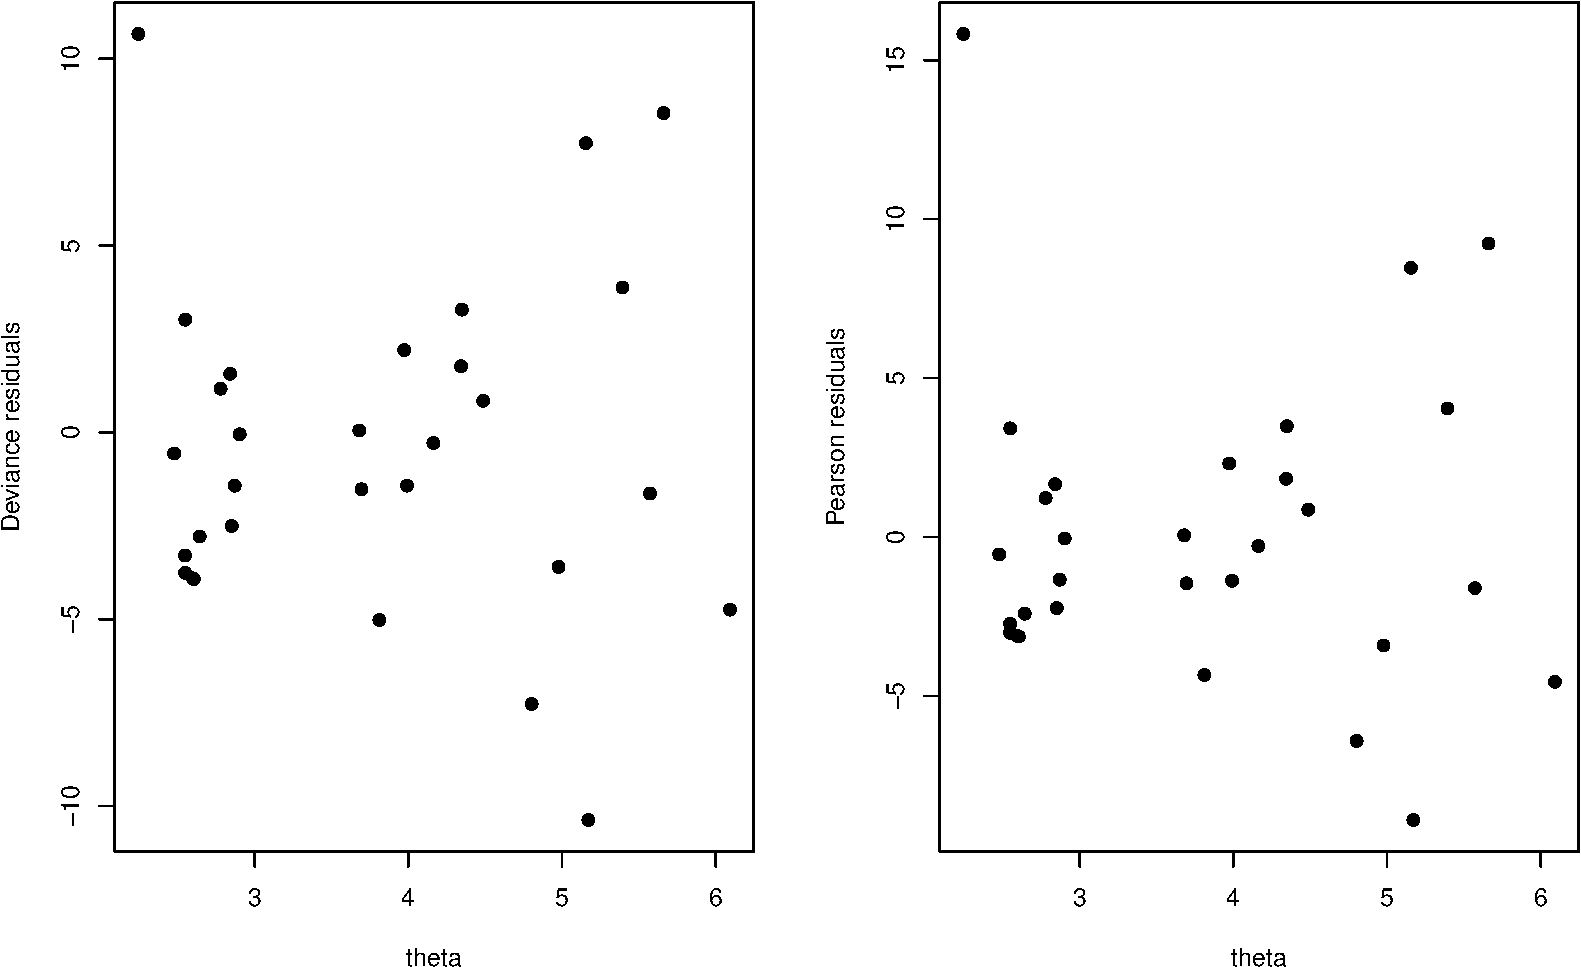
\includegraphics{week4_p2_files/figure-beamer/unnamed-chunk-19-1.pdf}
\end{frame}

\begin{frame}[fragile]{}
\protect\hypertarget{section-21}{}
\small

The relationship between the mean and the variance is shown below. A
line showing that the variance increases linearly in the mean (not a
perfect slope of 1) is also shown.

\vspace{12pt}
\tiny

\begin{Shaded}
\begin{Highlighting}[]
\FunctionTok{plot}\NormalTok{(}\FunctionTok{log}\NormalTok{(}\FunctionTok{fitted}\NormalTok{(m1)),}\FunctionTok{log}\NormalTok{((gala}\SpecialCharTok{$}\NormalTok{Species}\SpecialCharTok{{-}}\FunctionTok{fitted}\NormalTok{(m1))}\SpecialCharTok{\^{}}\DecValTok{2}\NormalTok{), }
     \AttributeTok{xlab=} \FunctionTok{expression}\NormalTok{(}\FunctionTok{hat}\NormalTok{(mu)),}\AttributeTok{ylab=}\FunctionTok{expression}\NormalTok{((y}\SpecialCharTok{{-}}\FunctionTok{hat}\NormalTok{(mu))}\SpecialCharTok{\^{}}\DecValTok{2}\NormalTok{), }\AttributeTok{pch =} \DecValTok{19}\NormalTok{)}
\FunctionTok{abline}\NormalTok{(}\DecValTok{0}\NormalTok{,}\DecValTok{1}\NormalTok{)}
\end{Highlighting}
\end{Shaded}

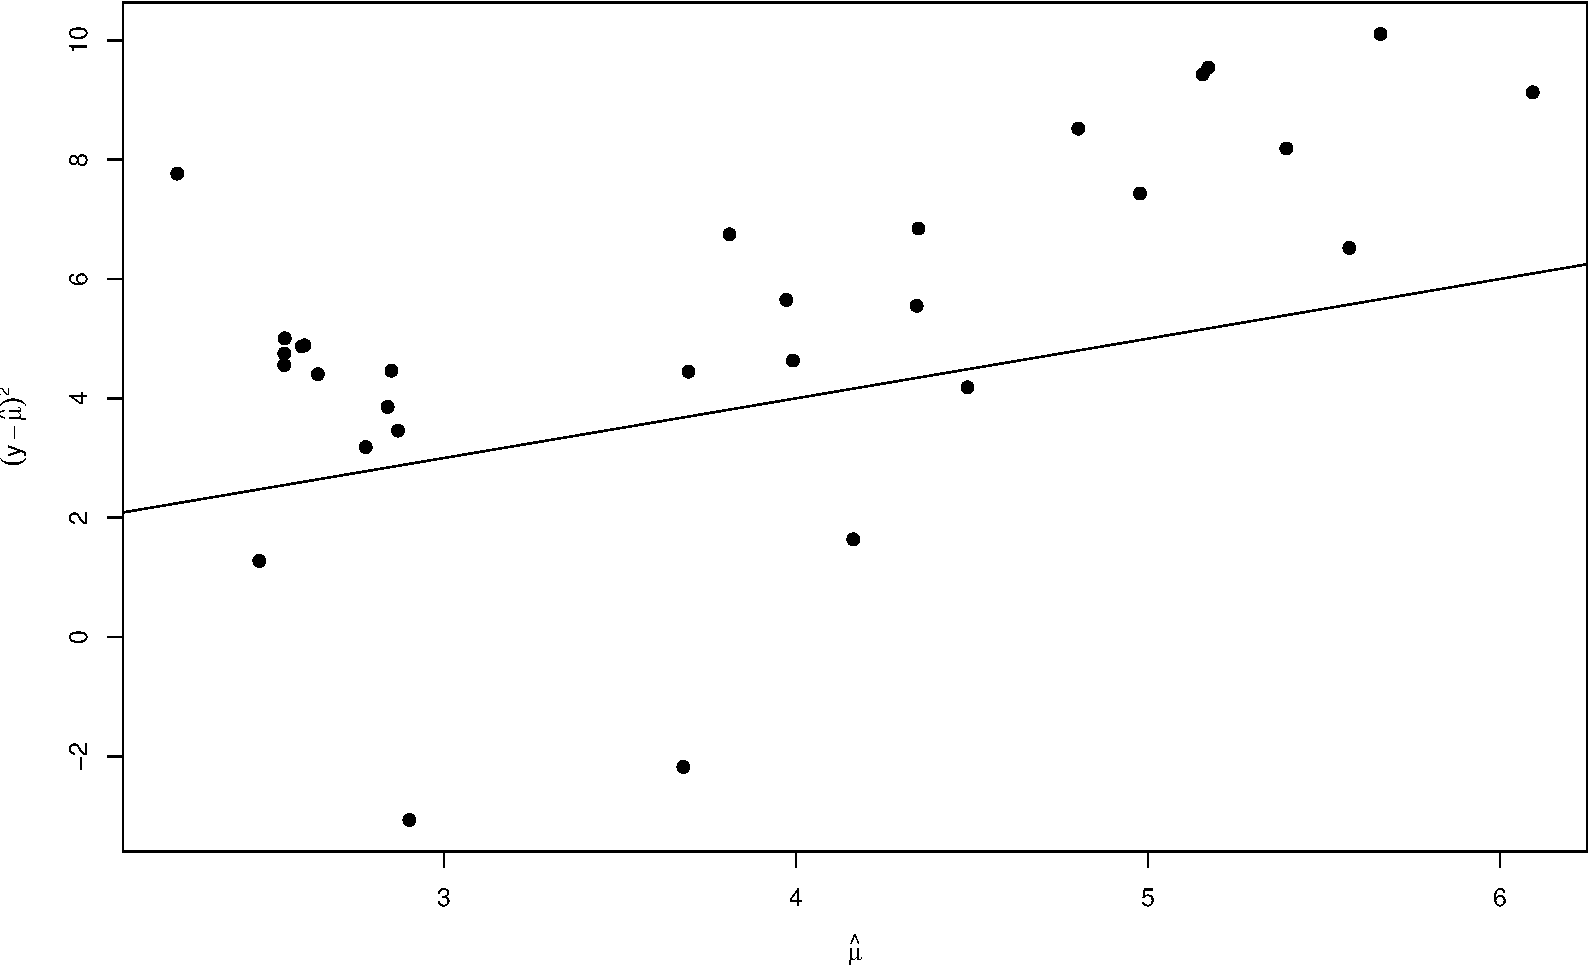
\includegraphics{week4_p2_files/figure-beamer/unnamed-chunk-20-1.pdf}
\end{frame}

\begin{frame}{}
\protect\hypertarget{section-22}{}
We see that the variance is proportional to, but larger than, the mean.

\vspace{12pt}

When the variance assumption of the Poisson regression model is broken
but the link function and choice of predictors are correct, the
estimates of \(\beta\) are consistent, but the standard errors will be
wrong.

\vspace{12pt}

This problem is called overdispersion.
\end{frame}

\begin{frame}[fragile]{(further reading)}
\protect\hypertarget{further-reading}{}
We note that a deviance based test tells us that our submodel does not
fit the data better than the full saturated model

\tiny

\begin{Shaded}
\begin{Highlighting}[]
\DocumentationTok{\#\# compare with saturated model}
\NormalTok{m1}\SpecialCharTok{$}\NormalTok{deviance}
\end{Highlighting}
\end{Shaded}

\begin{verbatim}
## [1] 594.1753
\end{verbatim}

\begin{Shaded}
\begin{Highlighting}[]
\NormalTok{m1}\SpecialCharTok{$}\NormalTok{df.residual}
\end{Highlighting}
\end{Shaded}

\begin{verbatim}
## [1] 23
\end{verbatim}

\begin{Shaded}
\begin{Highlighting}[]
\FunctionTok{pchisq}\NormalTok{(m1}\SpecialCharTok{$}\NormalTok{deviance, }\AttributeTok{df =}\NormalTok{ m1}\SpecialCharTok{$}\NormalTok{df.residual, }\AttributeTok{lower =} \ConstantTok{FALSE}\NormalTok{)}
\end{Highlighting}
\end{Shaded}

\begin{verbatim}
## [1] 7.617409e-111
\end{verbatim}
\end{frame}

\begin{frame}[fragile]{}
\protect\hypertarget{section-23}{}
The model misses bad in some spots

\vspace{12pt}
\tiny

\begin{Shaded}
\begin{Highlighting}[]
\NormalTok{foo }\OtherTok{\textless{}{-}} \FunctionTok{data.frame}\NormalTok{(}\AttributeTok{names =} \FunctionTok{rownames}\NormalTok{(gala),}
                  \AttributeTok{obs =}\NormalTok{ gala}\SpecialCharTok{$}\NormalTok{Species,}
                  \AttributeTok{pred =} \FunctionTok{as.numeric}\NormalTok{(}\FunctionTok{predict}\NormalTok{(m1, }\AttributeTok{type =} \StringTok{"response"}\NormalTok{)), }
                  \AttributeTok{resid =} \FunctionTok{residuals}\NormalTok{(m1))}
\FunctionTok{head}\NormalTok{(}\FunctionTok{cbind}\NormalTok{(foo }\SpecialCharTok{\%\textgreater{}\%} \FunctionTok{arrange}\NormalTok{(}\FunctionTok{desc}\NormalTok{(obs)) }\SpecialCharTok{\%\textgreater{}\%} \FunctionTok{pull}\NormalTok{(names),}
\NormalTok{           foo }\SpecialCharTok{\%\textgreater{}\%} \FunctionTok{arrange}\NormalTok{(}\FunctionTok{desc}\NormalTok{(pred)) }\SpecialCharTok{\%\textgreater{}\%} \FunctionTok{pull}\NormalTok{(names)), }\DecValTok{10}\NormalTok{)}
\end{Highlighting}
\end{Shaded}

\begin{verbatim}
##       [,1]           [,2]          
##  [1,] "SantaCruz"    "Isabela"     
##  [2,] "Isabela"      "SantaCruz"   
##  [3,] "SantaMaria"   "SanSalvador" 
##  [4,] "SanCristobal" "SanCristobal"
##  [5,] "SanSalvador"  "Baltra"      
##  [6,] "Pinzon"       "SantaMaria"  
##  [7,] "Pinta"        "Pinta"       
##  [8,] "Espanola"     "Marchena"    
##  [9,] "Fernandina"   "Espanola"    
## [10,] "Rabida"       "Pinzon"
\end{verbatim}
\end{frame}

\begin{frame}[fragile]{}
\protect\hypertarget{section-24}{}
\begin{Shaded}
\begin{Highlighting}[]
\NormalTok{foo }\SpecialCharTok{\%\textgreater{}\%} \FunctionTok{arrange}\NormalTok{(}\FunctionTok{desc}\NormalTok{(}\FunctionTok{abs}\NormalTok{(resid))) }\SpecialCharTok{\%\textgreater{}\%} \FunctionTok{head}\NormalTok{(}\DecValTok{10}\NormalTok{)}
\end{Highlighting}
\end{Shaded}

\begin{verbatim}
##                     names obs       pred      resid
## Gardner1         Gardner1  58   9.418902  10.662732
## Baltra             Baltra  58 176.259919 -10.372266
## SantaCruz       SantaCruz 444 287.434827   8.543845
## SantaMaria     SantaMaria 285 173.479088   7.741091
## Marchena         Marchena  51 121.814494  -7.267755
## Tortuga           Tortuga  16  45.214750  -5.018644
## Isabela           Isabela 347 442.973448  -4.741568
## Coamano           Coamano   2  13.517259  -3.923167
## Enderby           Enderby   2  13.421436  -3.902313
## SanCristobal SanCristobal 280 219.998697   3.879621
\end{verbatim}
\end{frame}

\begin{frame}[fragile]{}
\protect\hypertarget{section-25}{}
Can play around with the model to improve performance

\vspace{12pt}
\tiny

\begin{Shaded}
\begin{Highlighting}[]
\NormalTok{m3 }\OtherTok{\textless{}{-}} \FunctionTok{glm}\NormalTok{(Species }\SpecialCharTok{\textasciitilde{}}\NormalTok{ Elevation }\SpecialCharTok{+} \FunctionTok{I}\NormalTok{(Elevation}\SpecialCharTok{\^{}}\DecValTok{2}\NormalTok{) }\SpecialCharTok{+}\NormalTok{ Nearest }\SpecialCharTok{+}\NormalTok{ Scruz }\SpecialCharTok{+} 
            \FunctionTok{I}\NormalTok{(Scruz}\SpecialCharTok{\^{}}\DecValTok{2}\NormalTok{) }\SpecialCharTok{+}\NormalTok{ Adjacent }\SpecialCharTok{+} 
\NormalTok{            Area }\SpecialCharTok{+} \FunctionTok{I}\NormalTok{(Area}\SpecialCharTok{\^{}}\DecValTok{2}\NormalTok{), }\AttributeTok{family =} \StringTok{"poisson"}\NormalTok{, }\AttributeTok{data =}\NormalTok{ gala, }\AttributeTok{x =} \ConstantTok{TRUE}\NormalTok{)}

\NormalTok{foo }\OtherTok{\textless{}{-}} \FunctionTok{data.frame}\NormalTok{(}\AttributeTok{names =} \FunctionTok{rownames}\NormalTok{(gala),}
                  \AttributeTok{Species =}\NormalTok{ gala}\SpecialCharTok{$}\NormalTok{Species,}
                  \AttributeTok{pred =} \FunctionTok{as.numeric}\NormalTok{(}\FunctionTok{predict}\NormalTok{(m3, }\AttributeTok{type =} \StringTok{"response"}\NormalTok{)), }
                  \AttributeTok{resid =} \FunctionTok{residuals}\NormalTok{(m3))}
\FunctionTok{head}\NormalTok{(}\FunctionTok{cbind}\NormalTok{(foo }\SpecialCharTok{\%\textgreater{}\%} \FunctionTok{arrange}\NormalTok{(}\FunctionTok{desc}\NormalTok{(Species)) }\SpecialCharTok{\%\textgreater{}\%} \FunctionTok{pull}\NormalTok{(names),}
\NormalTok{           foo }\SpecialCharTok{\%\textgreater{}\%} \FunctionTok{arrange}\NormalTok{(}\FunctionTok{desc}\NormalTok{(pred)) }\SpecialCharTok{\%\textgreater{}\%} \FunctionTok{pull}\NormalTok{(names)), }\DecValTok{10}\NormalTok{)}
\end{Highlighting}
\end{Shaded}

\begin{verbatim}
##       [,1]           [,2]          
##  [1,] "SantaCruz"    "SantaCruz"   
##  [2,] "Isabela"      "Isabela"     
##  [3,] "SantaMaria"   "SanSalvador" 
##  [4,] "SanCristobal" "SanCristobal"
##  [5,] "SanSalvador"  "SantaMaria"  
##  [6,] "Pinzon"       "Pinta"       
##  [7,] "Pinta"        "Rabida"      
##  [8,] "Espanola"     "Marchena"    
##  [9,] "Fernandina"   "Fernandina"  
## [10,] "Rabida"       "Pinzon"
\end{verbatim}
\end{frame}

\begin{frame}[fragile]{}
\protect\hypertarget{section-26}{}
This model offers improvements in residual magnitude and we see that
problems are occurring for small species counts.

\vspace{12pt}
\tiny

\begin{Shaded}
\begin{Highlighting}[]
\NormalTok{foo }\SpecialCharTok{\%\textgreater{}\%} \FunctionTok{arrange}\NormalTok{(}\FunctionTok{desc}\NormalTok{(}\FunctionTok{abs}\NormalTok{(resid))) }\SpecialCharTok{\%\textgreater{}\%} \FunctionTok{head}\NormalTok{(}\DecValTok{11}\NormalTok{)}
\end{Highlighting}
\end{Shaded}

\begin{verbatim}
##                 names Species      pred     resid
## Gardner2     Gardner2       5  51.60949 -8.359204
## Gardner1     Gardner1      58  21.88658  6.389305
## Enderby       Enderby       2  26.28609 -6.186163
## Caldwell     Caldwell       3  27.87680 -6.031459
## SantaMaria SantaMaria     285 202.49381  5.459134
## Genovesa     Genovesa      40  15.30862  5.239687
## Coamano       Coamano       2  20.28438 -5.225127
## Espanola     Espanola      97  58.06115  4.656808
## Marchena     Marchena      51  89.57405 -4.438200
## Tortuga       Tortuga      16  38.53710 -4.116449
## Onslow         Onslow       2  14.26763 -4.083611
\end{verbatim}

\begin{Shaded}
\begin{Highlighting}[]
\FunctionTok{cbind}\NormalTok{(foo}\SpecialCharTok{$}\NormalTok{pred, gala[, }\SpecialCharTok{{-}}\DecValTok{8}\NormalTok{])[}\FunctionTok{which}\NormalTok{(}\FunctionTok{abs}\NormalTok{(foo}\SpecialCharTok{$}\NormalTok{resid) }\SpecialCharTok{\textgreater{}} \DecValTok{4}\NormalTok{), ]}
\end{Highlighting}
\end{Shaded}

\begin{verbatim}
##             foo$pred Species Endemics   Area Elevation Nearest Scruz Adjacent
## Caldwell    27.87680       3        3   0.21       114     2.8  58.7     0.78
## Coamano     20.28438       2        1   0.05        77     1.9   1.9   903.82
## Enderby     26.28609       2        2   0.18       112     2.6  50.2     0.10
## Espanola    58.06115      97       26  58.27       198     1.1  88.3     0.57
## Gardner1    21.88658      58       17   0.57        49     1.1  93.1    58.27
## Gardner2    51.60949       5        4   0.78       227     4.6  62.2     0.21
## Genovesa    15.30862      40       19  17.35        76    47.4  92.2   129.49
## Marchena    89.57405      51       23 129.49       343    29.1  85.9    59.56
## Onslow      14.26763       2        2   0.01        25     3.3  45.9     0.10
## SantaMaria 202.49381     285       73 170.92       640     2.6  49.2     0.10
## Tortuga     38.53710      16        8   1.24       186     6.8  50.9    17.95
\end{verbatim}
\end{frame}

\begin{frame}[fragile]{}
\protect\hypertarget{section-27}{}
\vspace{12pt}
\tiny

\begin{Shaded}
\begin{Highlighting}[]
\FunctionTok{plot}\NormalTok{(}\FunctionTok{log}\NormalTok{(}\FunctionTok{fitted}\NormalTok{(m3)),}\FunctionTok{log}\NormalTok{((gala}\SpecialCharTok{$}\NormalTok{Species}\SpecialCharTok{{-}}\FunctionTok{fitted}\NormalTok{(m3))}\SpecialCharTok{\^{}}\DecValTok{2}\NormalTok{), }
     \AttributeTok{xlab=} \FunctionTok{expression}\NormalTok{(}\FunctionTok{hat}\NormalTok{(mu)),}\AttributeTok{ylab=}\FunctionTok{expression}\NormalTok{((y}\SpecialCharTok{{-}}\FunctionTok{hat}\NormalTok{(mu))}\SpecialCharTok{\^{}}\DecValTok{2}\NormalTok{), }\AttributeTok{pch =} \DecValTok{19}\NormalTok{)}
\FunctionTok{abline}\NormalTok{(}\DecValTok{0}\NormalTok{,}\DecValTok{1}\NormalTok{)}
\end{Highlighting}
\end{Shaded}

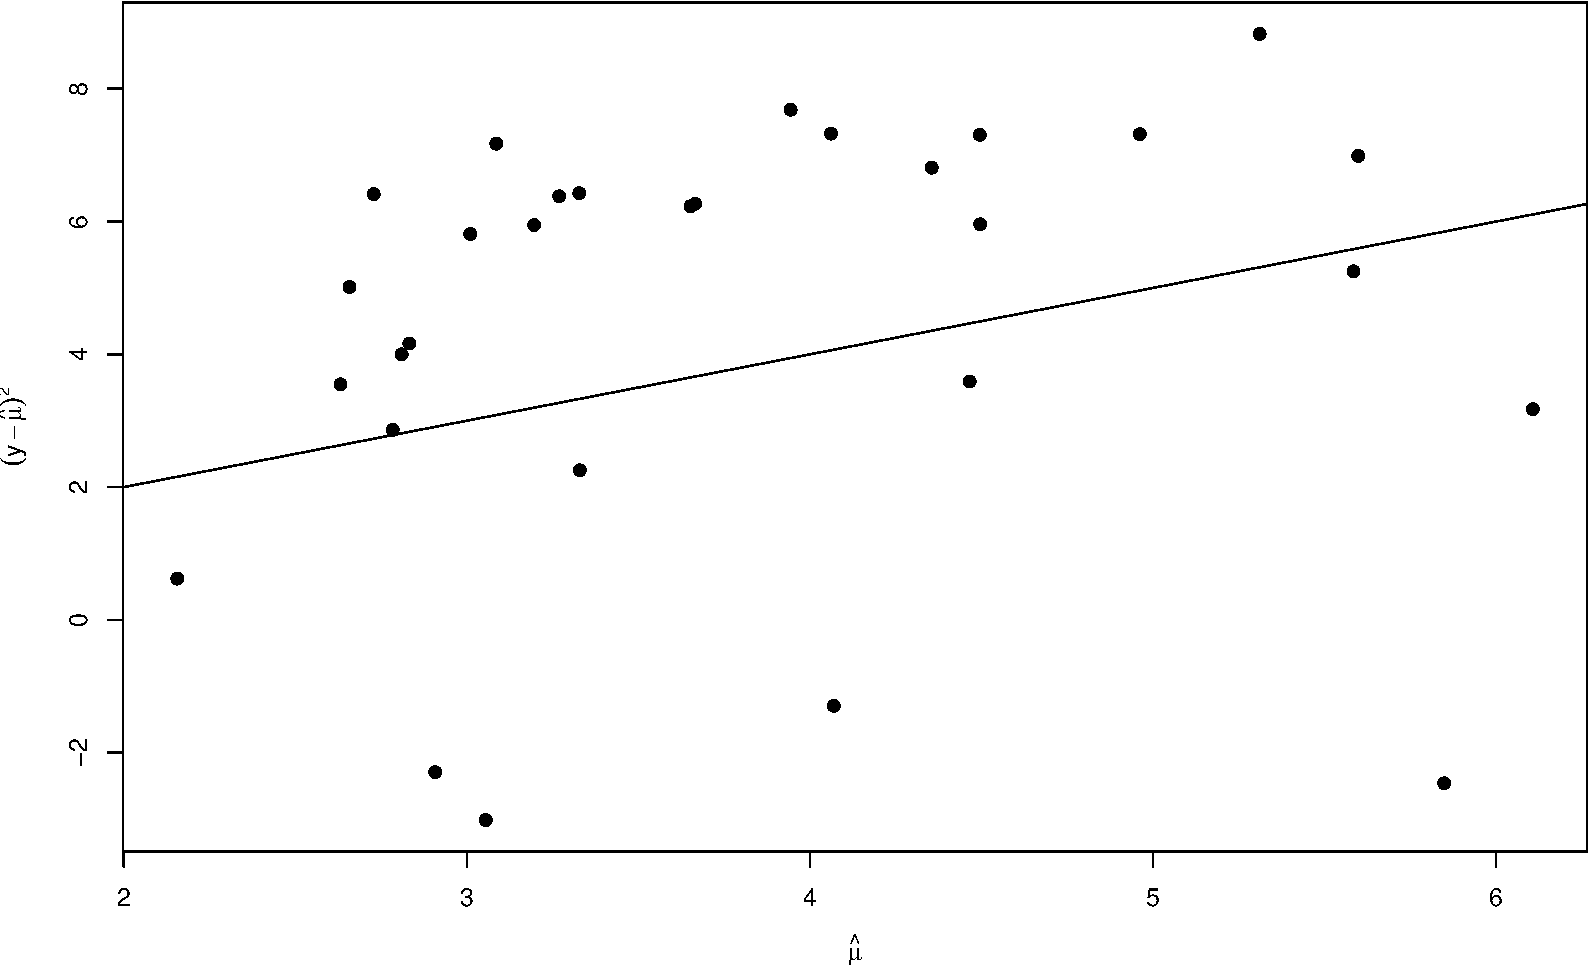
\includegraphics{week4_p2_files/figure-beamer/unnamed-chunk-27-1.pdf}

\begin{Shaded}
\begin{Highlighting}[]
\NormalTok{theta }\OtherTok{\textless{}{-}} \FunctionTok{as.numeric}\NormalTok{(m3}\SpecialCharTok{$}\NormalTok{x }\SpecialCharTok{\%*\%} \FunctionTok{coef}\NormalTok{(m3))}
\FunctionTok{par}\NormalTok{(}\AttributeTok{mfrow =} \FunctionTok{c}\NormalTok{(}\DecValTok{1}\NormalTok{,}\DecValTok{2}\NormalTok{))}
\FunctionTok{plot}\NormalTok{(theta, }\FunctionTok{residuals}\NormalTok{(m3), }\AttributeTok{xlab =} \StringTok{"theta"}\NormalTok{, }\AttributeTok{ylab =} \StringTok{"Deviance residuals"}\NormalTok{, }\AttributeTok{pch =} \DecValTok{19}\NormalTok{)}
\FunctionTok{plot}\NormalTok{(theta, }\FunctionTok{residuals}\NormalTok{(m3, }\StringTok{"pearson"}\NormalTok{), }\AttributeTok{pch =} \DecValTok{19}\NormalTok{,  }
     \AttributeTok{xlab =} \StringTok{"theta"}\NormalTok{, }\AttributeTok{ylab =} \StringTok{"Pearson residuals"}\NormalTok{)}
\end{Highlighting}
\end{Shaded}

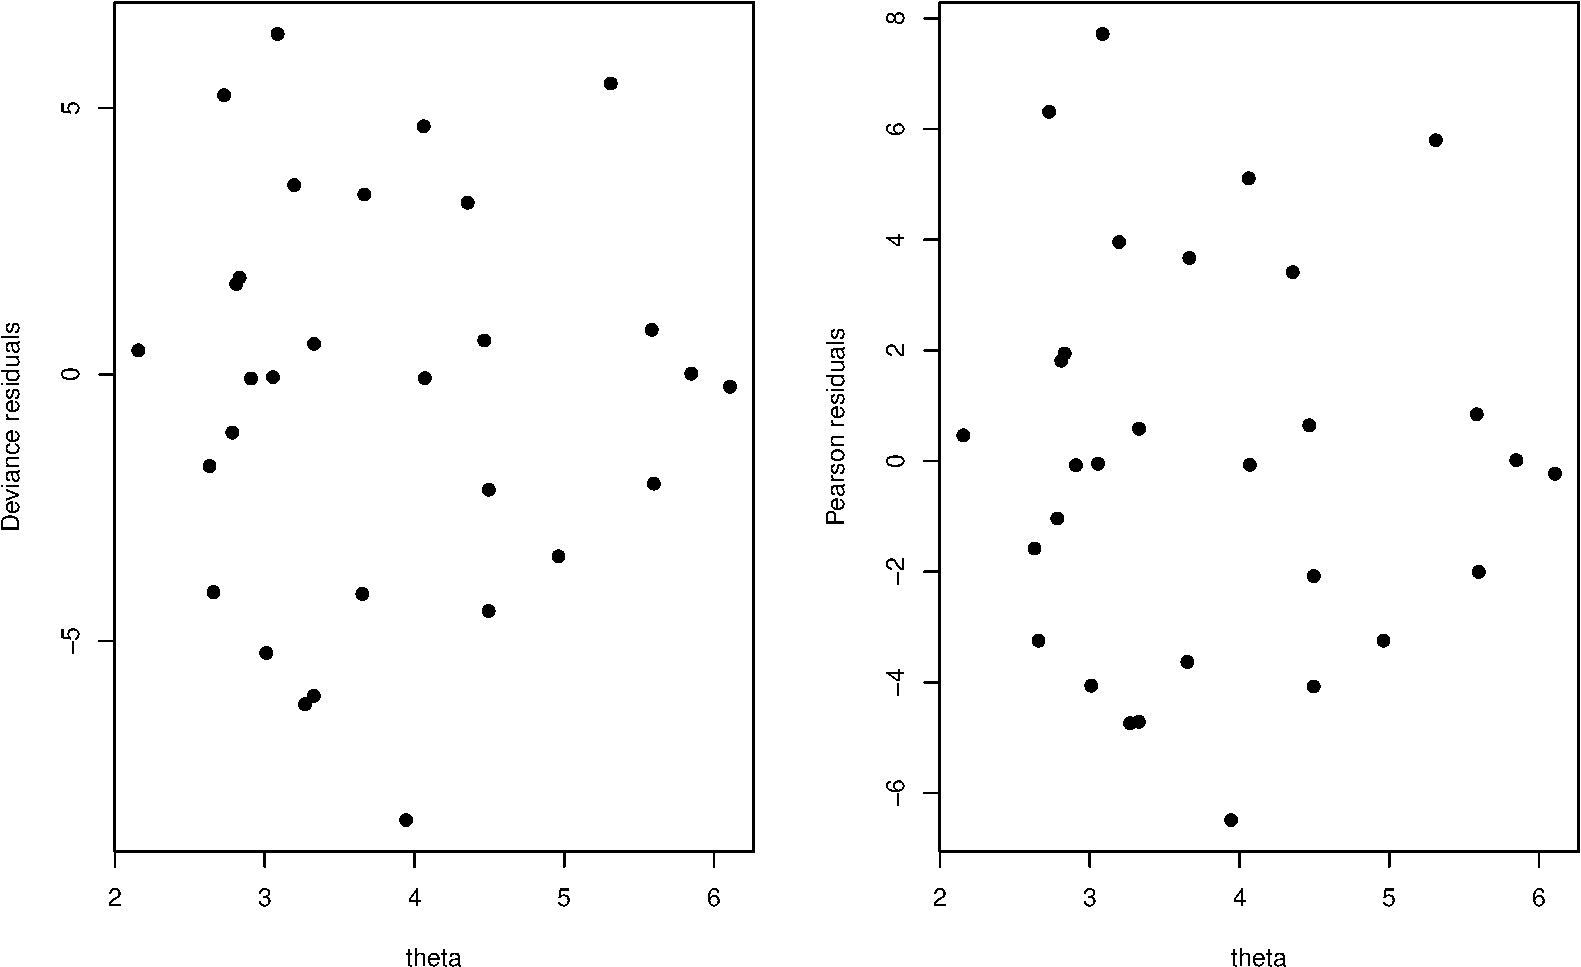
\includegraphics{week4_p2_files/figure-beamer/unnamed-chunk-28-1.pdf}
\end{frame}

\end{document}
